\documentclass[a4paper,11pt]{article}

\usepackage[T1]{fontenc}
\usepackage[utf8]{inputenc}
\usepackage{graphicx}
\usepackage{xcolor}
\usepackage[fleqn]{amsmath}
\usepackage{tgtermes}
\usepackage[final]{pdfpages}
\usepackage{wrapfig}

\usepackage[normalem]{ulem}
\useunder{\uline}{\ul}{}

\usepackage[
pdftitle={Lingwistyka Formalna i Automaty},
pdfauthor={evemorgen, AGH},
colorlinks=true,linkcolor=blue,urlcolor=blue,citecolor=blue,bookmarks=true,
bookmarksopenlevel=2]{hyperref}
\usepackage{amsmath,amssymb,amsthm,textcomp}
\usepackage{enumerate}
\usepackage{multicol}
\usepackage{tikz}
\usepackage{geometry}
\geometry{
 a4paper,
 total={170mm,257mm},
 left=20mm,
 top=20mm,
}

% custom footers and headers
\usepackage{fancyhdr,lastpage}
\pagestyle{fancy}
\lhead{}
\chead{}
\rhead{}
\lfoot{Assignment \textnumero{} 4}
\cfoot{}
\rfoot{Page \thepage\ /\ \pageref*{LastPage}}
\renewcommand{\headrulewidth}{0pt}
\renewcommand{\footrulewidth}{0pt}
%

%%%----------%%%----------%%%----------%%%----------%%%

\begin{document}

\title{Lingwistyka Formalna i Automaty - ćwiczenia 4}
\author{evemorgen, AGH}
\date{10/12/2016}
\maketitle

\newpage
\section{[DAS]}
\subsection{Ćwiczenie 2.2.1 a) i c) z książki „Wprowadzenie do teorii automatów języków i obliczeń” J. Hopcroft, R. Motwani, J. Ullman}
\subsection{Ćwiczenie 2.2.5 a), b), c) z książki „Wprowadzenie do teorii automatów języków i obliczeń” J. Hopcroft, R. Motwani, J. Ullman}

\section{Dane są języki: $L = \{0, 10, 111, 001\}, M = \{\varepsilon, 1, 01, 10\}$}
\subsection{wyznacz: $L^0, L^1, L^2$}
$L^0 = \{\varepsilon \}$ \\
$L^1 = LL^0 = \{0, 10, 111, 001\}$ \\
$L^2 = LL^1 = \{00, 010, 0111, 0001, 100, 1010, 10111, 10001, 0010, 00110, 001111, 001001 \}$
\subsection{wyznacz: $M^0, M^1, M^2, M^3$}
$M^0 = \{ \varepsilon \}$ \\
$M^1 = MM^0 = \{\varepsilon, 1, 01, 10\}$ \\
$M^2 = MM^1 = \{\varepsilon, 1, 01, 10, 11, 101, 110, 011, 0101, 0110, 1001, 1010 \}$ \\
$M^3 = MM^2 = \{\varepsilon, 1, 01, 10, 11, 101, 110, 011, 111, 0101, 0110, 1001, 1010, 1101, 1110, 1011, 10101, 10110, \\ 11001, 11010, 0111, 01101, 01110, 01011, 010101, 010110, 011001, 011010, 10011, 100101, 100110, 101001, 101010\}$

\subsection{wyznacz: $L^0 M^0, L^1 M^1, L^2 M^2$}
$L^0M^0 = \varepsilon \varepsilon = \varepsilon$ \\
$L^1 M^1 = \{0, 01, 10, 111, 001, 101, 1111, 0011, 1001, 11101, 00101, 010, 1010, 11110, 00110\}$ \\
$L^2 M^2 = moje życie jest za krótkie żeby rozpisywać to gówno$

\section{Jakim językiem będzie $L^*$ dla:}
\subsection{L = \{a,b\}}
$L^* = \{a,b,aa,ab,ba,bb, aaa,aab,aba,abb,baa,bab,bba,bbb,...\}$
\subsection{L = \{a, bb\}}
$l^* = {a, "bb", aa, a"bb", "bb"a, "bb""bb", aaa, aa"bb", ...}$

\newpage
\section{Ile elementów posiada język $L^i$ jeśli:}
\subsection{L = \{a,b\}}
$len(\{a,b\}) ** i \leftrightarrow 2 ** i$
\subsection{L = \{a,b,c\}}
$len(\{a,b\}) ** i \leftrightarrow 3 ** i$
\subsection{L= \{ 1,2,..,n\}}
$len(\{1,2,..,n\}) ** i \leftrightarrow n ** i$

\section{Czy języki $L^i$ z poprzedniego zadania są skończone czy nie? A język $L^*$?}

Języki $L^i$ są skończone, języki $L^*$ z definicji są nie skończone

\section{Dany jest język L będący zbiorem wszystkich łańcuchów złożonych z 'a' (w tym z łańcuchazawierającego zero symboli 'a').}
\subsection{Czy język ten jest skończony?}
Nie, ten język nie jest skończony.
\subsection{Jakim językiem będzie $L^*$?}
$L^* = L$, $|L| \rightarrow \infty$

\section{Podaj przykład języka (regularnego) dla którego $L^*$ nie jest nieskończone.}
$L = \{\varepsilon\}$

\newpage
\section{Zapisać wyrażenie regularne reprezentujące język:}
\subsection{będący zbiorem łańcuchów zaczynającym się o '1' po którym następuje jedno lub więcej '0' i kończący się '1'}
$100^*1$
\subsection{będący zbiorem wszystkich łańcuchów w których na zmianę występuje '1' i '0'}
$((1+\varepsilon)01(01)^*(0+\varepsilon)) + (0+\varepsilon)10(10)^*(1+\varepsilon))$
\subsection{będący zbiorem łańcuchów stanowiących literały całkowitoliczbowe ósemkowe i szesnastkowe o dowolnej długości zapisywane zgodnie z konwencją języka Java.}
Osemki = (0(1+2+3+4+5+6+7)(1+2+3+4+5+6+7)*) \\
Szesnastki = (0X(1+2+3+4+5+6+7+8+9+A+B+C+D+E+F)(1+2+3+4+5+6+7+8+9+A+B+C+D+E+F)*) \\
Rozw = Osemki + Szesnastki
\subsection{będący zbiorem łańcuchów przedstawiających numery NIP w formacie XXX-XXX-XX-XX lub XXX-XX-XX-XXX (gdzie X oznacza dowolną cyfrę 0-9)}
C = (0+1+2+3+4+5+6+7+8+9)  \\
Rozw = CCC-CCC-CC-CC + CCC-CC-CC-CCC
\subsection{będący zbiorem wszystkich łańcuchów nad alfabetem {a,b,c} zawierającym co najmniej jedno a i jedno b}
$(a+b+c)^*a(a+b+c)^*b(a+b+c)^* + (a+b+c)^*b(a+b+c)^*a(a+b+c)^*$
\subsection{będący zbiorem wszystkich łańcuchów nad alfabetem {0,1} w których jedynka jest na 8 pozycji od prawej}
$(0+1)^*1(0+1)(0+1)(0+1)(0+1)(0+1)(0+1)(0+1)$

\newpage
\section{Zakładając że alfabet $\Sigma = \{0,1\}$ określ jakie języki reprezentują poszczególne wyrażenia regularne}
\subsection{$0^*10^*$}
Język zawierający słowa zawierające dowolną ilość zer,  jedynkę a następnie znowu dowolną ilość zer
\subsection{$\Sigma^*1 \Sigma^*$ (przez $\Sigma$ rozumiemy wystąpienie dowolnego znaku alfabetu – czyli 0+1)}
Język zawierający słowa które posiadają conajmniej jedną jedynkę i składają się tylko z zer i jedynek
\subsection{$\Sigma^*001 \Sigma ^*$}
Język zawierający słowa posiadające podciąg 001 i składające się tylko z zer i jedynek
\subsection{$(\Sigma \Sigma)^*$}
Język zawierający słowa których długość jest wielokrotnością 2 i składają się z samych zer i jedynek
\subsection{$\Sigma \Sigma ^*$}
Język zawierający słowa których długość jest  >= 1  oraz składają się z samych zer i jedynek
\subsection{$\Sigma ^* \Sigma ^*$}
Język zawierający słowa których długość jest  >= 0 oraz składają się z samych zer i jedynek
\subsection{01+10}
Język składający się ze słów 01 oraz 10
\subsection{$1+\emptyset$ (gdzie $\emptyset$ – zbiór pusty)}
Język posiadający jedno słowo "1"
\subsection{$1\emptyset$}
Język posiadający jedno słowo $\varepsilon$
\subsection{$\emptyset^*$}
Język posiadający jedno słowo $\varepsilon$


\newpage
\section{Zamienić poniższe wyrażenia regularne na $\varepsilon$-NAS}
\subsection{01*0}
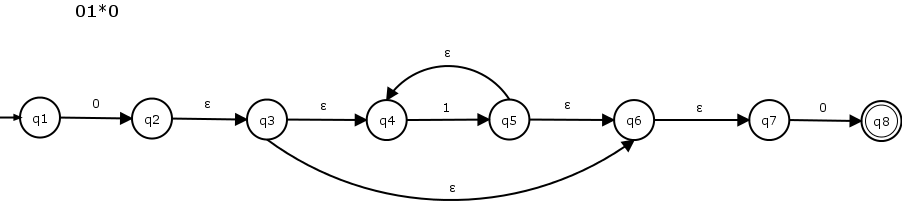
\includegraphics[scale=0.5]{10-1}
\subsection{(0+1)10}
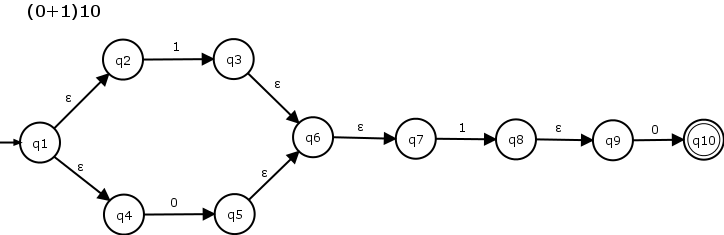
\includegraphics[scale=0.6]{10-2}
\subsection{aa(a+b)*b}
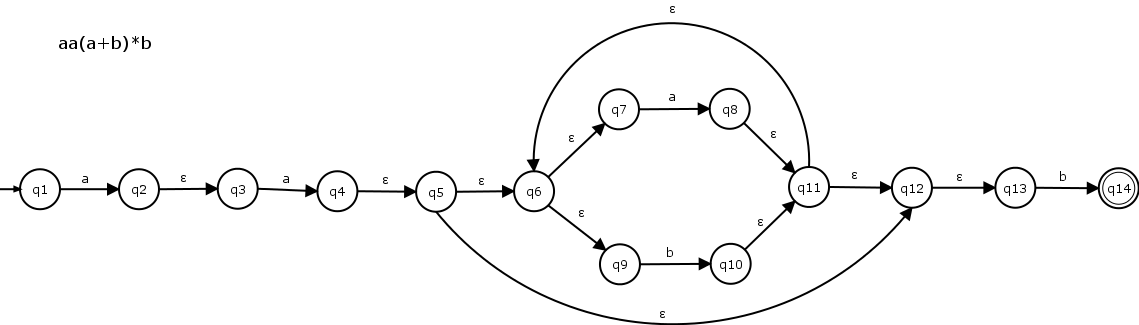
\includegraphics[scale=0.4]{10-3}

\section{Przekonwertować poszczególne $\varepsilon$-NAS z poprzedniego zadania na DAS.}
$moje życie jest za krótkie żeby konwertować to długie gównpo$


\end{document}
